\documentclass[tikz,border=10pt]{standalone}
\usepackage{tikz}
\usepackage{amsmath}
\usetikzlibrary{shapes.geometric,positioning,arrows.meta,calc,patterns}

\begin{document}
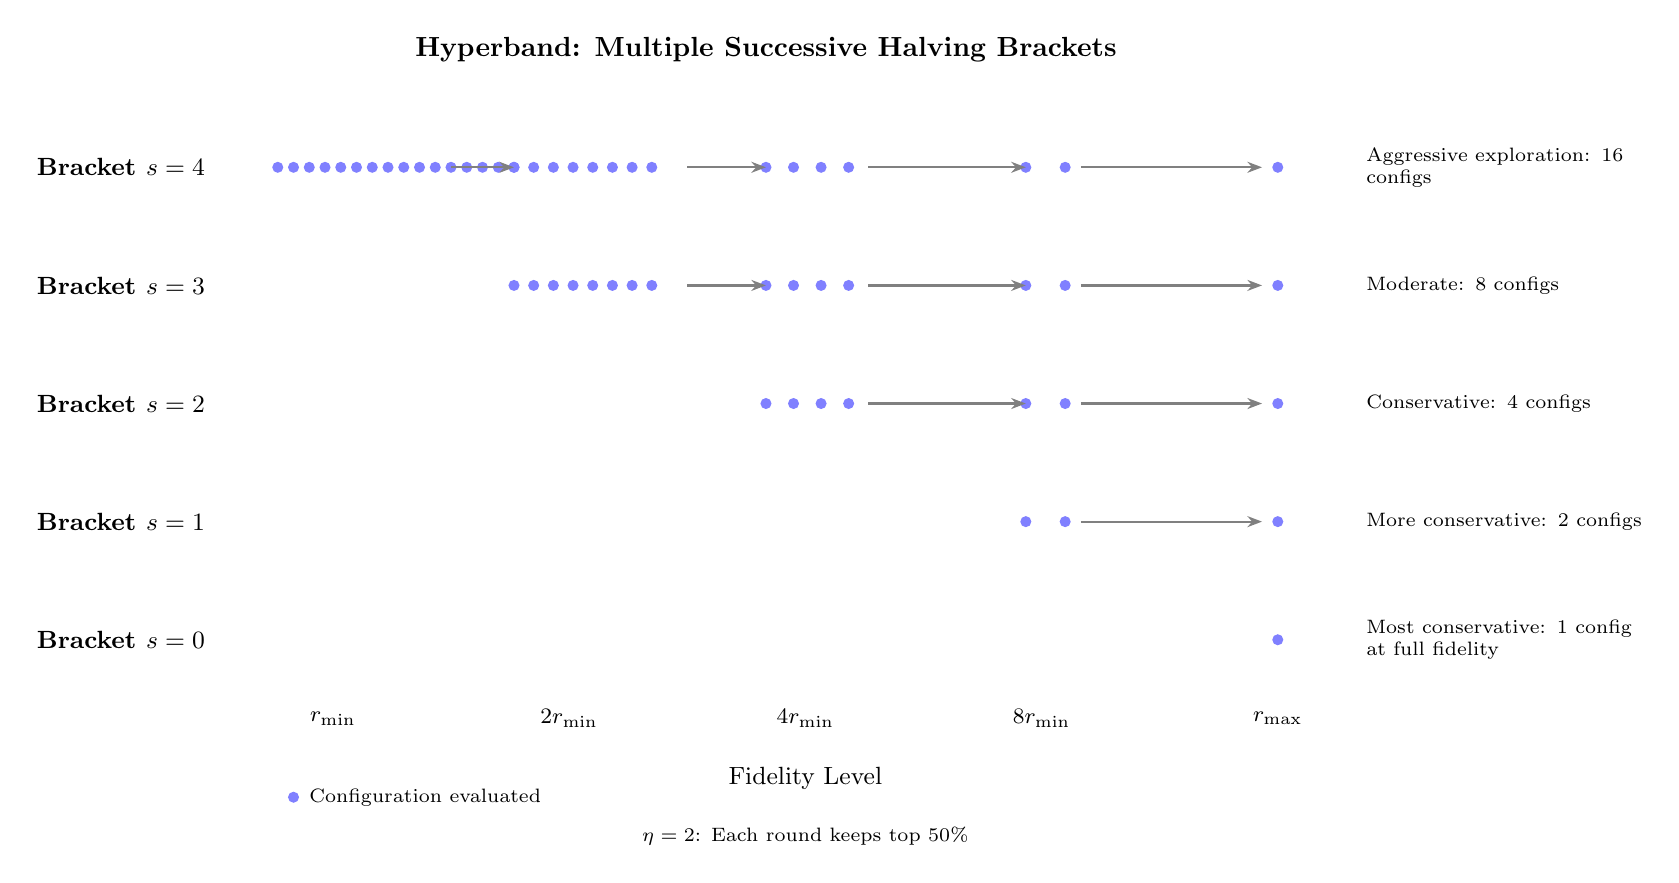
\begin{tikzpicture}[
    bracket/.style={draw, thick, rounded corners=2pt, minimum height=0.6cm},
    config/.style={circle, fill=blue!50, minimum size=4pt, inner sep=0},
    elim/.style={circle, fill=red!30, minimum size=4pt, inner sep=0},
    arrow/.style={-{Stealth[scale=0.8]}, thick, gray}
]

% Title
\node[font=\bfseries] at (6.5, 5.5) {Hyperband: Multiple Successive Halving Brackets};

% Bracket labels
\node[anchor=east, font=\small\bfseries] at (-0.5, 4) {Bracket $s=4$};
\node[anchor=east, font=\small\bfseries] at (-0.5, 2.5) {Bracket $s=3$};
\node[anchor=east, font=\small\bfseries] at (-0.5, 1) {Bracket $s=2$};
\node[anchor=east, font=\small\bfseries] at (-0.5, -0.5) {Bracket $s=1$};
\node[anchor=east, font=\small\bfseries] at (-0.5, -2) {Bracket $s=0$};

% Fidelity labels (bottom)
\node[font=\footnotesize] at (1, -3) {$r_{\min}$};
\node[font=\footnotesize] at (4, -3) {$2r_{\min}$};
\node[font=\footnotesize] at (7, -3) {$4r_{\min}$};
\node[font=\footnotesize] at (10, -3) {$8r_{\min}$};
\node[font=\footnotesize] at (13, -3) {$r_{\max}$};
\node[font=\small, anchor=north] at (7, -3.5) {Fidelity Level};

% Bracket s=4: Most aggressive (many configs, low initial fidelity)
\foreach \i in {1,...,16} {
    \pgfmathsetmacro{\x}{0.3 + (\i-1)*0.2}
    \node[config] at (\x, 4) {};
}
\foreach \i in {1,...,8} {
    \pgfmathsetmacro{\x}{3.3 + (\i-1)*0.25}
    \node[config] at (\x, 4) {};
}
\foreach \i in {1,...,4} {
    \pgfmathsetmacro{\x}{6.5 + (\i-1)*0.35}
    \node[config] at (\x, 4) {};
}
\foreach \i in {1,...,2} {
    \pgfmathsetmacro{\x}{9.8 + (\i-1)*0.5}
    \node[config] at (\x, 4) {};
}
\node[config] at (13, 4) {};

% Bracket s=3
\foreach \i in {1,...,8} {
    \pgfmathsetmacro{\x}{3.3 + (\i-1)*0.25}
    \node[config] at (\x, 2.5) {};
}
\foreach \i in {1,...,4} {
    \pgfmathsetmacro{\x}{6.5 + (\i-1)*0.35}
    \node[config] at (\x, 2.5) {};
}
\foreach \i in {1,...,2} {
    \pgfmathsetmacro{\x}{9.8 + (\i-1)*0.5}
    \node[config] at (\x, 2.5) {};
}
\node[config] at (13, 2.5) {};

% Bracket s=2
\foreach \i in {1,...,4} {
    \pgfmathsetmacro{\x}{6.5 + (\i-1)*0.35}
    \node[config] at (\x, 1) {};
}
\foreach \i in {1,...,2} {
    \pgfmathsetmacro{\x}{9.8 + (\i-1)*0.5}
    \node[config] at (\x, 1) {};
}
\node[config] at (13, 1) {};

% Bracket s=1
\foreach \i in {1,...,2} {
    \pgfmathsetmacro{\x}{9.8 + (\i-1)*0.5}
    \node[config] at (\x, -0.5) {};
}
\node[config] at (13, -0.5) {};

% Bracket s=0: Most conservative (few configs, high initial fidelity)
\node[config] at (13, -2) {};

% Arrows showing progression
\draw[arrow] (2.5, 4) -- (3.3, 4);
\draw[arrow] (5.5, 4) -- (6.5, 4);
\draw[arrow] (7.8, 4) -- (9.8, 4);
\draw[arrow] (10.5, 4) -- (12.8, 4);

\draw[arrow] (5.5, 2.5) -- (6.5, 2.5);
\draw[arrow] (7.8, 2.5) -- (9.8, 2.5);
\draw[arrow] (10.5, 2.5) -- (12.8, 2.5);

\draw[arrow] (7.8, 1) -- (9.8, 1);
\draw[arrow] (10.5, 1) -- (12.8, 1);

\draw[arrow] (10.5, -0.5) -- (12.8, -0.5);

% Annotations
\node[anchor=west, font=\scriptsize, text width=3.5cm] at (14, 4) {Aggressive exploration: 16 configs};
\node[anchor=west, font=\scriptsize, text width=3.5cm] at (14, 2.5) {Moderate: 8 configs};
\node[anchor=west, font=\scriptsize, text width=3.5cm] at (14, 1) {Conservative: 4 configs};
\node[anchor=west, font=\scriptsize, text width=3.5cm] at (14, -0.5) {More conservative: 2 configs};
\node[anchor=west, font=\scriptsize, text width=3.5cm] at (14, -2) {Most conservative: 1 config at full fidelity};

% Legend
\node[config, label={[font=\scriptsize]right:Configuration evaluated}] at (0.5, -4) {};
\node[font=\scriptsize] at (7, -4.5) {$\eta = 2$: Each round keeps top 50\%};

\end{tikzpicture}
\end{document}
